\section{TPM}
\subsection{Principe de chiffrement symétrique, asymétrique, fonction de hachage et signature digitale}
\subsubsection{Chiffrement symétrique}
Cipher=chiffrement, connu de tout le monde (AES, CHACHA20, ...)
La même clé est utilisée pour l'encryption que la decryption. Le cleartext est découpé en block, chaque block a la même longueur (64, 128bits) et chaque block est encrypté avec un algo (AES, IDEA, ...) et une clé. CBC: chaque block est encodé avec le résultat du précédent c'est un XOR bit par bit entre IV (connu pour le premier) et le bit à encoder.
\begin{Verbatim}[breaklines=true, breakanywhere=true]
# encrypt a file
openssl enc -aes-256-cbc -e -in t.txt -out t.enc
# decrypt a file
openssl enc -aes-256-cbc -d -in t.enc -out t.txt
\end{Verbatim}
\subsubsection{Chiffrement asymétrique}
La clé d'encryption (publique ou privée) n'est pas la même que celle de decryption (publique ou privée). Algo: Elliptical Curves, RSA, DSA, ... et c'est très lent.
Alice et Bob doivent échanger le clé publique. 
Sans digital signature: Bob doit encrypter avec la public key de Alice et elle va la décryptée avec sa clé privée. Avec digital signature: Bob encrypte avec sa clé privée et Alice décode avec sa clé publique.
\begin{Verbatim}[breaklines=true, breakanywhere=true]
# compute private-public keys
openssl genrsa -out rsa_key.pem 2048
# get public key
openssl rsa -in rsa_key.pem -pubout -out rsa_key_pub.pem
# show private-public keys
openssl rsa -in rsa_key.pem –text
# show public key
openssl rsa -in rsa_key_pub.pem –pubin –text
# encrypt t.txt with public key
openssl rsautl -encrypt -pubin -inkey rsa_key_pub.pem -in t.txt -out t.rsa
# decrypt t.rsa with private key
openssl rsautl -decrypt -inkey rsa_key.pem -in t.rsa -out t1.txt
\end{Verbatim}
\subsubsection{Fonction de hachage}
Une fonction $H$ qui prend une entrée $m$ de n'importe quelle taille et qui génère $h$ qui est une fixed-size string (according to md5, sha512). 2 $m$ différentes ne devraient jamais donnée la même sortie $h$ sinon c'est une collision (catastrophique).
\begin{Verbatim}[breaklines=true, breakanywhere=true]
md5sum file
a6a0e8d0522e2c5de921b1c455506320
\end{Verbatim}
\subsubsection{Signature digitale}
Objectif : intégrité du message et authentification de l'origine du message. 
%2 steps: une hash function qui va créer l'empreinte du message et cette empreinte va être encrypté par un asymetric cipher et une clé privée. Bob reçoit le message est en clair avec la signature. Il va passer le message dans un cipher et comparer le résultat à la décryption de la signature à l'aide de la clé publique d'Alice.
\begin{figure}[H]
\centering
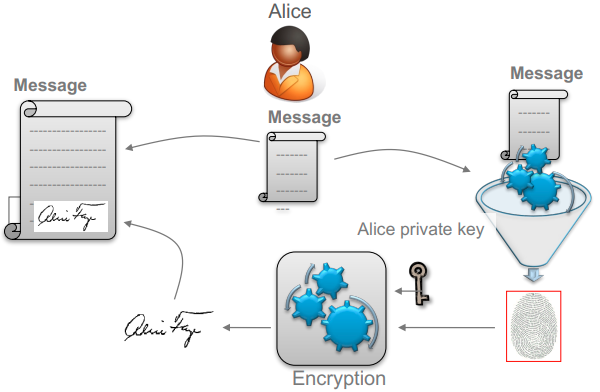
\includegraphics[width=0.9\columnwidth]{Figures/tpm_01.png}
\end{figure}
\begin{Verbatim}[breaklines=true, breakanywhere=true]
# 3 même ligne que Asym cipher
# sign t.txt with public key
openssl dgst -sha256 -sign rsa_key.pem -out t.sign t.txt
# decrypt t.rsa with private key
openssl dgst -verify -sha256 rsa_key_pub.pem -signature t.sign t.txt
\end{Verbatim}
\subsection{Différentes implémentations des TPM}
Discrete: Implémentation dans le semidconductor d'un chip dédié.
Integrated: Partie d'un chip, ex ARM: TrustZone.
Hypervisor:Virtual TPMs provided by and rely on hypervisors.
Software:Emulator software avec pas plus de protection qu'un os.
\subsection{Architecture interne d'un TPM}
Il contient des algo asym et sym, des fonctions de hash, des random generator, des key generator, de la NV Ram (persistent), des PCR (platform configuration register) et de la RAM classique.
\subsection{Hiérarchies des TPM}
Endorsement: réservé pour des objet créés et certifiés par le manufacturer (la eseed est gen randomly at manufacture time et ne bougera jamais (peut servir d'ID)). Platform: réservé pour des objets créés par le OEM qui construit la plateforme (la pseed est gen randomly at manufacture time mais peut être changée : \verb!tmp2_changepps!). Owner hierarchy: reserved for us, on peut regen la oseed avec \verb!tpm2_clear!. Null hierarchy: réservé pour des clés éphémères qui sont regénérées at reboots. Toutes les clés (peut importe la hiérachie sont générées avec des Key Derivation Function). Les TPMS génère des clé qui sont à base de true random source et ces clés ne quittent que le TPM de manière crypté par sa clé parent.

\subsection{Créer et utiliser des TPM}
\begin{center}
\verb!tpm2_createprimary -C <A> -G rsa2048 -c <B>.ctx!\\
\begin{tabular}{cc}
$<$A$>$ & $<$B$>$ \\\hline
e & \verb!e_primary!\\
p & \verb!p_primary!\\
o & \verb!o_primary!\\
n & \verb!n_primary!
\end{tabular}
\end{center}

\subsection{Commandes principales}
\begin{lstlisting}[style=bash]
tpm2_getcap handles-transient #voir clé dans la RAM
tpm2_getcap handles-persistent #voir clé dans la NV-RAM
tpm2_evictcontrol -c o_primary.ctx # sauver une clé en NV-RAM
tpm2_readpublic ... # pour lire la clé publique et ensuite utiliser openssh pour la voir
tpm2_flushcontext! -t ##effacer toute la RAM
tpm2_create -C o_prim -G rsa2048 -u child_pub -r child_priv #créer clé enfant
tpm2_load -C o_prim -u child_pub -r child_priv -c child #charger clé enfant
shred passwd, rm -f passwd #supprimer de l'hôte

\end{lstlisting}

\subsection{encrypter-décrypter, signer-vérifier}
\begin{lstlisting}[style=bash]

tpm2_rsaencrypt -c child -s rsaes clearfile -o encryptedfile
tpm2_rsadecrypt -c child -s rsaes encryptedfile -o clearfile
tpm2_sign -c child -g sha256 -o file.sign file
tpm2_verifysignature -c child -g sha256 -s file.sign -m file
\end{lstlisting}

\subsection{PCR}
Tout registrer est chaque fois hash pour chaque modification. Un update est appelé extend. La specification de la plateforme TPM spécifie les PCR attributes et ou va quoi est standardizé.
\begin{lstlisting}[style=bash]
tpm2_pcrreset 0
tpm2_pcrextend 0:sha1=8c83...(hash)
\end{lstlisting}

\subsection{Sauver des données sur le TPM}
On va par exemple créer un mot de passe, le sauver sur le TPM, le supprimer sur le host et le récupérer quand il y besoin.
\begin{lstlisting}[style=bash]
tpm2_evictcontrol -c passwd.ctx 0x81010000 -C o  #sauver
tpm2_unseal -c 0x81010000 > passwd  #récuperer
\end{lstlisting}

\subsection{Sauver des données sur le TPM et les protéger avec une PCR policy}
Par exemple unseal data seulement si les valeurs des registres PCV n'ont pas changé (pas eu de tentative de hacking).
\begin{lstlisting}[style=bash]
sha1sum passwd #calcul hash
tpm2_pcrreset 0 #flush PCR0
tpm2_pcrextend 0:sha1=8c839... #sauve hash
tpm2_createprimary -C o -G rsa2048 -c primary
tpm2_startauthsession -S session
tpm2_policypcr -S session -l sha1:0 -L pcr0_policy #créer politique
tpm2_flushcontext session

tpm2_create -C primary -g sha256 \
-u passwd_pcr0.pub -r passwd_pcr0.priv \
-i passwd -L pcr0_policy

tpm2_evictcontrol -c passwd_pcr0 0x81010000 -C o
tpm2_flushcontext session

shred passwd
rm -f passwd

tpm2_startauthsession --policy-session -S session
tpm2_policypcr -S session -l sha1:0
tpm2_unseal -p session:session -c 0x81010000 > passwd
\end{lstlisting}


